
\documentclass[a4paper, 11pt]{article}

\usepackage[margin=2cm]{geometry}

\usepackage{amsfonts, amsmath, amssymb, amsthm}
%\usepackage{graphicx}
\usepackage{tikz}
\usepackage{hyperref}
\usepackage[caption=false]{subfig}


\numberwithin{equation}{section}

\theoremstyle{plain}
\newtheorem{theorem}	[equation]	{Theorem}
\newtheorem{conjecture}	[equation]	{Conjecture}
\newtheorem{corollary}	[equation]	{Corollary}
\newtheorem{definition}	[equation]	{Definition}
\newtheorem{example}	[equation]	{Example}
\newtheorem{lemma}		[equation]	{Lemma}
\newtheorem{problem}	[equation]	{Problem}
\newtheorem{proposition}[equation]	{Proposition}
\newtheorem{remark}		[equation]	{Remark}

\theoremstyle{definition}
\newtheorem{claim}		[equation]	{Claim}
\newtheorem{exercise}   {Exercise}  [section]
\newtheorem{answer}     {Answer}    [section]

\usepackage[noend]{algpseudocode}
\usepackage{algorithm}

\newcommand{\GF}{\mathrm{GF}}
\newcommand{\rk}{\mathrm{rk}}
\newcommand{\id}{\mathrm{id}}
\newcommand{\dH}{d_\mathrm{H}}
\newcommand{\dmin}{d_{\min}}
\newcommand{\wH}{w_\mathrm{H}}
\newcommand{\wmin}{w_{\min}}
\newcommand{\lcm}{\mathrm{lcm}}

\newcommand{\N}{\mathbb{N}}
\newcommand{\Z}{\mathbb{Z}}
\newcommand{\Q}{\mathbb{Q}}
\newcommand{\R}{\mathbb{R}}

\renewcommand{\i}{\mathrm{i}}
\newcommand{\e}{\mathrm{e}}

\newcommand{\divides}{\,|\,}

\newcommand{\probability}{\mathbb{P}}
\newcommand{\expectation}{\mathbb{E}}


	\newcommand{\Important}[1]{\textcolor{red}{#1}}
	\newcommand{\Structure}[1]{\textcolor{blue}{#1}}
	\newcommand{\Reference}[1]{\textcolor{teal}{#1}}
	\newcommand{\Define}[1]{\textcolor{purple}{#1}}


\newcommand{\alphabet}[1]{\mathcal{#1}}

\newcommand{\code}[1]{\mathsf{#1}}
\newcommand{\Paritycheck}           {\code{PC}}
\newcommand{\Repetition}            {\code{R}}
\newcommand{\Hamming}               {\code{H}}
\newcommand{\Golay}                 {\code{G}}
\newcommand{\ReedMuller}            {\code{RM}}
\newcommand{\ReedSolomon}           {\code{RS}}
\newcommand{\GeneralizedReedSolomon}{\code{GRS}}
\newcommand{\Alternant}             {\code{A}}
\newcommand{\Goppa}                 {\code{\Gamma}}


\renewcommand{\thesection}{\arabic{section}}

% Change date format to use it for version number
\usepackage[yyyymmdd]{datetime}
\renewcommand{\dateseparator}{.}


\title{Data Compression}
\date{Version \today}
\author{lrfk99}

\begin{document}

\maketitle


\section{Statistical compression I: Huffman coding}
\label{sec:01}


\subsection{Prefix codes}

\paragraph{Memoryless sources}

We have some data that we wish to encode. It could be anything: Spoken English, Data from a digital camera sensor, DNA string, etc.

We model our data as coming from a memoryless source $X$. We imagine that symbols are emitted at random according to the probability distribution of $X$. In other words, we view our data as a random string $X_1, X_2, \dots$ over some alphabet $\mathcal{X}$. Our memoryless assumption is that those form a sequence of independent identically distributed (i.i.d.) random variables: $X_i \sim X$ for all $i$.

More concretely, for any $x \in \mathcal{X}$ and any $i$, the probability 
\[
    \probability(X_i = x)
\]
is independent of $i$, and of all previous or future emitted symbols.

Note that this is not always a valid assumption. We will look into source modelling into more detail in the next lectures.

\paragraph{The coding problem}

We have a source emitting symbols in $\mathcal{X} = \{x_1, \dots, x_n\}$ with respective probabilities  $\{p_1, \dots, p_n\}$.

Question: If  $\mathcal{D}$ is an alphabet of  $D$ code symbols, how can we encode the source symbols using code words (finite strings of code symbols) as economically as possible?

Formally: a \Define{source code} is a map $C : \mathcal{X} \to \mathcal{D}^*$
where  $\mathcal{D}^*$     is the set of all finite strings of symbols in  $\mathcal{D}$.

The words $C(x)$ are called the \Define{codewords}, and the integers $|C(x)|$ (the length of $C(x)$) are the \Define{word lengths}.

We can extend the code to messages as follows. A \Define{message} is any finite string of source symbols $m = m_1 \dots m_k \in \mathcal{X}^*$ and its encoding is the obvious concatenation 
\[
    C(m) = C(m_1) C(m_2) \dots C(m_k).
\]

\paragraph{Prefix codes}


A code $C$ is \Define{uniquely decodable} (a.k.a. uniquely decipherable) if every finite string in $\mathcal{D}^*$ is the image of at most one message. 

A prefix of a word $w = w_1 \dots w_k \in \mathcal{D}^*$ is any word of the form $w_1 \dots w_l$ for some $0 \le l \le k$ (for $l=0$, we obtain the empty word). A code is \Define{prefix} (a.k.a. instantaneous or prefix-free) if there are no two distinct source symbols $x, y \in \mathcal{X}$ such that $C(x)$ is a prefix of  $C(y)$         .

\begin{theorem}
A prefix code is uniquely decodable.
\end{theorem}

\begin{proof}
Let $C$ be a prefix code, and let $w = C(m)$ for some message $m = m_1 \dots m_k \in \mathcal{X}^*$. We give a decoding algorithm which, given $w$, determines $m$. Let $w = w_1 \dots w_l$.

Let $i$ be the smallest integer such that $w_1 \dots w_i$ is a codeword, say $w_1 \dots w_i = C(x)$. Then the $m_1 = x$. Indeed, if $m_1 = y \ne x$, then $C(x)$ is a prefix of $C(y)$, which is a contradiction. Then repeat this step, beginning with $w_{i+1}$ and hence determining $m_2$, and so on until $w$ is empty.
\end{proof}

\begin{example}
Let $\mathcal{X} = \{a, b, c, d, e\}$, $\mathcal{D} = \{0,1\}$ and 
\begin{align*}
    C(a) &= 01\\
    C(b) &= 100\\
    C(c) &= 101\\
    C(d) &= 1101\\
    C(e) &= 1111.
\end{align*}

Suppose we need to decode the word $C(m) = w = 10010111011111100101$. We proceed as follows. We read the word until we reach a codeword:
\begin{align*}
    w_1 &= 1\\
    w_1 w_2 &= 10\\
    w_1 w_2 w_3 &= 100 = C(b). 
\end{align*}
Therefore $m_1 = b$. We continue until we reach a codeword:
\begin{align*}
    w_4 &= 1\\
    w_4 w_5 &= 10\\
    w_4 w_5 w_6 &= 101 = C(c). 
\end{align*}
Therefore $m_2 = c$. And so on... Exercise \ref{exercise:prefix} asks you to finish this simple example.
\end{example}


\subsection{Huffman codes}


\paragraph{Compact codes}

Our main aim is to design codes where the typical length of messages is reduced dramatically. The basic idea is to assign short codewords to more frequent symbols and longer codewords to less frequent ones.


More formally, the \Define{average length} (a.k.a. expected length) of the code is 
\[
    L(C) = \expectation( |C(X)| ) = \sum_{x \in \mathcal{X}} |C(x)| \probability(X = x).
\]

A code is \Define{compact} (for a given source $X$) if it is uniquely decodable and it minimises the average length of codewords over all uniquely decodable codes.


\begin{theorem}
A uniquely decodable code with prescribed word lengths exists if and only if a prefix code with the same word lengths exists.
\end{theorem}


\begin{corollary}
For any source $X$, there is a compact prefix code for $X$.
\end{corollary}


\paragraph{Binary Huffman code}


The key is to construct a tree where the leaves correspond to the symbols in  $\mathcal{X}$ and the paths from the root to the leaves give the codewords.

The tree is constructed iteratively. Suppose $\mathcal{X} = \{x_1, \dots, x_n\}$ with $p_1 \ge p_2 \ge  \dots \ge p_{n-1} \ge p_n$. Then merge $x_{n-1}$ and $x_n$ into a new symbol, say $x_{n-1, n}$ with probability $p_{n-1} + p_n$, and let $x_{n-1}$ and $x_n$ be the children of $x_{n-1, n}$ on the tree. Label the edges from $x_{n-1, n}$ to its children as $0$ and $1$, respectively. Repeat for the new source $X^{(1)} = \{x_1, \dots, x_{n-2}, x_{n-1, n} \}$ (making sure to order the symbols in non-decreasing probability). Repeat until the final source $X^{(n-1)}$ only has one symbol left with probability $1$; that symbol is the root of the tree. 

Once the tree is built, read off the labels on the path from the root to a leaf to get the corresponding codeword.

\begin{example} \label{example:huffman}
Let $X$ with respective probabilities $a: 0.4, b: 0.2, c: 0.15, d:0.15, e:0.1$.

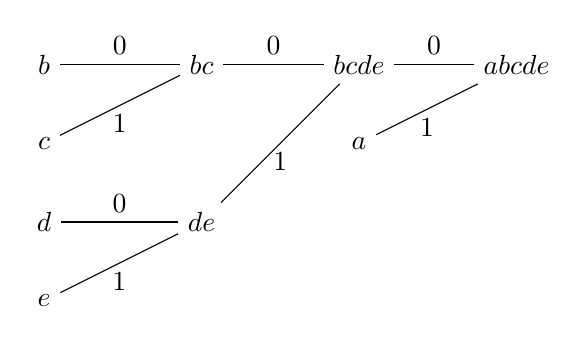
\begin{tikzpicture}[xscale=2]
    %\node (a0) at (0,4) {$a$}; %0.4
    %\node (b0) at (0,3) {$b$}; %0.2
    %\node (c0) at (0,2) {$c$}; %0.15
    \node (d0) at (1,2) {$d$}; %0.15
    \node (e0) at (1,1) {$e$}; %0.1
    
    %\node (a1) at (1,4) {$a$}; %0.4
    %\node (de1) at (1,3) {$de$}; %0.25
    \node (b1) at (1,4) {$b$}; %0.2
    \node (c1) at (1,3) {$c$}; %0.15
    
    %\node (a2) at (2,4) {$a$}; %0.4
    \node (bc2) at (2,4) {$bc$}; %0.35
    \node (de2) at (2,2) {$de$}; %0.25

    \node (bcde3) at (3,4) {$bcde$}; %0.6
    \node (a3) at (3,3) {$a$}; %0.4

    \node (abcde4) at (4,4) {$abcde$}; %1

\draw (de2) -- node[above] {$0$} ++(d0);
\draw (de2) -- node[below] {$1$} ++(e0);

\draw (bc2) -- node[above] {$0$} ++(b1);
\draw (bc2) -- node[below] {$1$} ++(c1);

\draw (bcde3) -- node[above] {$0$} ++(bc2);
\draw (bcde3) -- node[below] {$1$} ++(de2);

\draw (abcde4) -- node[above] {$0$} ++(bcde3);
\draw (abcde4) -- node[below] {$1$} ++(a3);


\end{tikzpicture}

The code is then
\begin{align*}
    C(a) &= 1\\
    C(b) &= 000\\
    C(c) &= 001\\
    C(d) &= 010\\
    C(e) &= 011
\end{align*}
The average length is then $2.2$ bits per symbol.
\end{example}


Note that there is no need for general tie-breaking rules. Indeed, different merges may yield different codes, and maybe even different code lengths, but always the same expected length. Similarly, the assignment of $0$ or $1$ does not change the code lengths.

\paragraph{Huffman codes are compact} Clearly, Huffman codes are prefix. The proof that they are compact is by induction on the number of symbols and omitted. It can be found in \cite[Section 5.8]{CT06}.


\paragraph{Non-binary Huffman codes}

Huffman codes can be extended to non-binary alphabets: If we have an alphabet of $D$ characters, we group the $D$ least likely symbols at each stage of reducing the source. When expanding the code we append each of the $D$ characters to one of the least likely symbols’ codewords.

We must end up with exactly $D$ symbols in the final source, so we may need to pad the original source up to $D+k(D-1)$ by adding symbols of probability $0$.

\subsection{See further}

\paragraph{Codes and Automata} The mathematical theory of uniquely decodable codes is reviewed in \cite{BPR10}, where they are simply referred to as codes. The language generated by a prefix code can be recognised by very a simple deterministic finite automaton; in fact, the relation between codes and automata is very deep and explored throughout the book. Note that this book hardly talks about data compression!

\paragraph{Canonical Huffman codes} As we shall see in Exercise \ref{exercise:huffman_unequal_lengths}, there can be several different Huffman trees for the same source. However, there is always a so-called canonical Huffman tree (and hence code) with a special shape that can be easily computed; see \cite[3.2.2]{Say12}.

\paragraph{Adaptive Huffman coding} Huffman coding is based on a source $X$ with given probabilities. In general, the probability of an element is computed by its relative frequency in the message; for instance, if the message has 100 characters, 34 of them are ``e'', then the probability of ``e'' is 34\%. Computing those probabilities then requires scanning the whole document before building the tree. Adaptive Huffman coding, on the other hand, builds the Huffman tree as the document is scanned, making small updates (if any) each time a new character is scanned.

\subsection{Exercises}

\begin{exercise} \label{exercise:not_prefix}
Let $\mathcal{X} = \{x_1, \dots, x_q\}$ for $q \ge 2$. Give a binary code $C : \mathcal{X} \to \{0,1\}^*$ that is uniquely decodable but neither prefix nor suffix.
\end{exercise}

\begin{exercise} \label{exercise:prefix}
Finish the example of decoding a prefix code.
\end{exercise}

\begin{exercise} \label{exercise:decoding_prefix}
How could you make the decoding algorithm of prefix codes more efficient? Would you use that modification for decoding Huffman codes? How would you include the decision problem: given $w \in \mathcal{D}^*$, determine whether $w$ is a codeword.
\end{exercise}

\begin{exercise} \label{exercise:huffman}
Construct a binary Huffman code for $X$ with probabilities $0.5, 0.2, 0.15, 0.1, 0.05$. What is the average length, and how does it compare with the one in Example \ref{example:huffman}?
\end{exercise}

\begin{exercise} \label{exercise:huffman_unequal_lengths}
Let $X$ have probabilities $(1/3, 1/3, 1/4, 1/{12})$. Show that, depending on how you merge, the binary Huffman coding procedure may lead to different code lengths, namely $(2,2,2,2)$ or $(1,2,3,3)$. Verify that the average length remains the same, though.
\end{exercise}



\section{Statistical compression II: Arithmetic coding} 
\label{sec:02}

%\subsection{Adaptive Huffman coding}


\subsection{Arithmetic coding}


\paragraph{Limitation of Huffman coding} Consider a source with a heavily imbalanced distribution: say $a :0.99$ and $b: 0.01$. Suppose we want to encode the sequence 
\[
    m = aaaaaaaaaa
\]
(of length $10$) using Huffman coding. Then we would require $10$ bits (the length of the message). 

However, if you compute the probability of that particular $10$-character sequence, we get 
\[
    p(m) = p(a)^{10} \approx 0.904.
\]
So if we were to compute the Huffman code based on all $2^{10}$ possible sequences, $m$ would be encoded as only one bit!

The main limitation of Huffman is then apparent: the codewords are only defined for symbols, not messages. Arithmetic coding offers a way of working at the \Important{sequence level}, thereby assigning a particular tag to any sequence, without working out all the tags for all sequences of the same length.

Suppose $X = \{a_1, \dots, a_n\}$ with respective probabilities $p_1, \dots, p_n$. We want to encode the message $m = a_{i_1} \dots a_{i_k}$. The output of the arithmetic encoder will be a \Important{number} in the range $[0,1)$ that uniquely describes $m$.

\begin{example} \label{example:arithmetic}
Let $X = \{a_1, a_2, a_3\}$ with probabilities $p_1 = 0.4, p_2 = 0.5, p_3 = 0.1$. The interval $[0,1)$ is subdivided among the three symbols as 
\[
    a_1 : [0, 0.4), \quad a_2 : [0.4, 0.9), \quad a_3 : [0.9, 1). 
\]
The interval is then recursively subdivided in the same fashion, e.g. $a_1 : [0, 0.4)$ is subdivided into 
\[
    a_1a_1 : [0, 0.16), \quad a_1a_2 : [0.16, 0.36), \quad a_1a_3 : [0.36, 0.4). 
\]
The final code for $a_1a_3$ could be any number in the range $[0.36, 0.4)$. The decoding is performed by iteratively performing the splits and choosing the interval where the code belongs. For instance, say we send $c = 0.36$ (obviously, we only send $36$), then the decoder first finds out that $c \in [0, 0.4)$ hence $m_1 = a_1$; then $c \in [0.36, 0.4)$ hence $m_2 = a_2$.
\end{example}




For each symbol processed, the current interval gets smaller and requires more bits to express it, but the final output is a single number for the whole sequence, which is not simply the concatenation of the codewords for its symbols. We illustrate the encoding and decoding processes in more detail by using a slightly more complex example.



We show the compression steps for the string ``SWISS\textvisiblespace MISS''. This time, the probabilities directly arise from the character frequencies, which are computed as a preliminary step to the encoding process.\\
~\\

\begin{tabular}{l|l|l|l}
    Character $x$    & Frequency  & Probability          & Range  $[L(x), H(x) )$     \\
    \hline
    S       & 5     & 0.5    & [0.5, 1.0)         \\ 
    W       & 1     & 0.1    & [0.4, 0.5)         \\ 
    I       & 2     & 0.2    & [0.2, 0.4)         \\ 
    M       & 1     & 0.1    & [0.1, 0.2)         \\ 
    \textvisiblespace       & 1     & 0.1     & [0.0, 0.1)       
\end{tabular}
~\\
~\\

The encoding process begins by defining two variables $Low$ and $High$ and setting them to $0$ and $1$, respectively.They define an interval $[Low, High)$. As symbols are being input and processed, the values of $High$ and $Low$ are moved closer together. As the symbol $x$ is being input and processed, $Low$ and $High$ are updated according to
\begin{align*}
    High    &\gets Low + (High - Low) H(x),\\
    Low     &\gets Low + (High - Low) L(x).
\end{align*}
~\\

\begin{tabular}{l|l|l|l|l}
    $x$   & $L(x)$  & $H(x)$  & $Low$     & $High$     \\
    \hline
        &       &       & 0     & 1     \\
    S   & 0.5   & 1.0     & 0.5   & 1.0     \\
    W   & 0.4   & 0.5   & 0.70   & 0.75     \\
    I   & 0.2   & 0.4   & 0.71   & 0.72     \\
    S   & 0.5   & 1.0     & 0.715   & 0.72     \\
    S   & 0.5   & 1.0     & 0.7175   & 0.72     \\
    \textvisiblespace   & 0.0   & 0.1     & 0.7175   & 0.71775     \\
    M   & 0.1   & 0.2   & 0.717525   & 0.717550     \\
    I   & 0.2   & 0.4   & 0.717530   & 0.717535     \\
    S   & 0.5   & 1.0     & 0.7175325   & 0.717535     \\
    S   & 0.5   & 1.0     & 0.71753375   & 0.717535     
\end{tabular}
~\\

The final code is the final value of $Low$, $0.71753375$ of which only the eight digits $71753375$ need to be written.


The decoder first inputs the symbols and their range, and reconstructs the table of frequencies and probabilities. It then inputs the rest of the code. The first digit is $7$, so the number is $0.7\ldots \in [0.5, 1)$: the first symbol is then S. It carries on, updating the code number to remove the effect of the character it just input. More explicitly, after the character $x$, it performs the update
\[
    C \gets \frac{C - L(x)}{H(x) - L(x)}.
\]
The decoder carries on until $C = 0$, in which case there should be a way to make it stop (either an end-of-file symbol is part of the input, or the length of the input was given in the header of the code).\\
~\\

\begin{tabular}{l|l|l|l}
    $x$   & $L(x)$      & $H(x)$      & $C$     \\
    \hline
        &           &           & 0.71753375     \\
    S   & 0.5       & 1.0       & 0.4350675     \\
    W   & 0.4       & 0.5       & 0.350675     \\
    I   & 0.2       & 0.4      & 0.753375     \\
    S   & 0.5      & 1.0      & 0.50675     \\
    S   & 0.5      & 1.0      & 0.0135     \\
    \textvisiblespace   & 0.0      & 0.1      & 0.135     \\
    M   & 0.1      & 0.2      & 0.35     \\
    I   & 0.2      & 0.4      & 0.75     \\
    S   & 0.5      & 1.0      & 0.5     \\
    S   & 0.5      & 1.0      & 0     
\end{tabular}


\subsection{Implementation details}

\paragraph{Using integers} The encoding as described before is not practical, since it uses numbers of unlimited precision for $Low$ and $High$. The decoder process is also impractical: the number $C$ can be a very long integer.


Any practical implementation of arithmetic coding should only use integers and should not be very long. Here is an implementation that uses integers with only four digits (We only give the encoder, but the decoder can be worked out as ``doing the same in reverse,'' as we are getting used to seeing.)

The main idea is that once the leftmost digits of $Low$ and $High$ are equal, then they remain equal henceforth. So we should ``forget about'' the leftmost digit once the encoder has output it. This is done by shifting the digits. Using four digits, we first initialise $L^* = 0000$ (corresponding to $Low = 0.0000\dots = 0$) and $H^* = 9999$ (corresponding to $High = 0.9999\dots = 1$), and we proceed as follows.\\
~\\

\begin{tabular}{l|l|l|l|l|l}
    $x$   & $Low$     & $High$     & Digit & $L^*$ & $H^*$ \\
    \hline
        & 0     & 1     &       & 0000  & 9999 \\
    S   & 0.5   & 1     &       & 5000  & 9999 \\
    W   & 0.7   & 0.75  & 7     & 0000  & 4999 \\
    I    & 0.1 & 0.2 &  1     & 0000  & 9999 \\
    S    & 0.5 & 1.0 &       & 5000  & 9999 \\
    S    & 0.75 & 1.0 &       & 7500  & 9999 \\
    \textvisiblespace    & 0.75 & 0.775 &  7    & 5000  & 7499 \\
    M    & 0.525 & 0.55 &  5     & 2500  & 4999 \\
    I    & 0.3 & 0.35 & 3      & 0000  & 4999 \\
    S    & 0.25 & 0.5 &       & 2500  & 4999 \\
    S    & 0.375 & 0.5 & 3750   &   & 4999  
\end{tabular}
~\\

In this toy example, we used four digits, but in practice we should be using enough to make sure that enough information is conveyed by $H^*$ and $L^*$ at all times. Another potential issue is that of underflow, when for instance $High$ decreases too fast and loses its significant digits. Scaling is then performed to avoid this situation.

\paragraph{Using binary strings} Firstly, note that we can choose to output any number in the range $[Low, High)$, ans not necessarily $Low$ per se. A certain choice of value may have fewer digits in its binary expansion, and hence require less space than $Low$. Moreover, obviously operations should be carried out in binary instead of decimal.

It can be shown that, if one uses the number $(Low + High)/2$, then one only needs to transmit the first
\[
    l = \left\lceil \log \frac{1}{p(m)} \right\rceil + 1
\]
bits of that number, where $p(m)$ is the probability of the input sequence $m$. This is very close to optimality indeed.

\subsection{Exercises}

\begin{exercise} \label{exercise:arithmetic}
With the same source as in Example \ref{example:arithmetic}, encode the message $m = a_2a_3a_1a_1a_3$.
\end{exercise}



\begin{exercise} \label{exercise:swiss_miss}
Work out a decoder for the four-digit implementation of arithmetic coding, and decode the output of the SWISS MISS example.
\end{exercise}


% \subsection{Answers}



\section{Lempel-Ziv I: LZ77}
\label{sec:03}


\subsection{Limitations of statistical compression}

In Lectures \ref{sec:01} and \ref{sec:02} we looked at compact codes for data being emitted by a memoryless source - a random process.

This week we look at encoding a fixed file of data efficiently. Rather than having estimates for the probabilities of each symbol, we can look at the whole message and determine the frequency of each symbol. Compact codes for memoryless sources are guaranteed to be optimal on average, but we may not have an average message. If the encoding is not determined in advance (as can be done for known sources), but is message dependent, then we must transmit the code as well as the encoded message.

Recall, memoryless sources emit each symbol independently of any previous symbols. There is no ‘pattern’ to the data beyond the frequency of each symbol. For instance, consider the message 
\[
    abbaeadcaadccbaabaaa
\]
(20 characters). The letter frequencies are a:10/20, b:4/20, c:3/20, d:2/20, e:1/20. These agree exactly with the probabilities in Exercise \ref{exercise:huffman}. Using the Huffman code $abbaeadcaadccbaabaaa$ becomes
\[
    100001011110110010110110010010001100111
\]
(39 characters, as expected - 1.95 bits on average). 

It is not obvious that we can do better here, and in general for randomly chosen messages with these frequencies we simply can't! But what about: 
\[
    aaaaaaaaaabbbbcccdde
\]
or: 
\[
    ababababacacacadadae ?
\]
Again, Huffman coding would yield 39 characters. Clearly, those messages have more than just statistical redundancy; they also have a form of structural redundancy to which statistical methods such as Huffman coding are oblivious.





\paragraph{Source modelling}

A lot of work was done in the early days of text compression to model natural languages and to understand their redundancy. The first work is Shannon's statistical analysis of English text \cite{Sha51}, and it has been significantly refined over the years (see Cover and King \cite{CK78} for a survey of techniques). 

Using a completely different approach, Zipf \cite{Zip49} exhibited a remarkable variety of hyperbolic laws in social sciences; in particular the distribution of words in a natural language approximately satisfies the beautiful law described below. Suppose a natural language has $N$ words, sorted in non-increasing frequency ($p(1) \ge p(2) \ge \dots p(r) \dots \ge p(N)$). Then the probability of the word at the $r$-th rank is
\[
    p(r) = \frac{ \mu }{ r },
\]
with
\[
    \mu \approx \frac{ 1 }{ \log_e N + \gamma },
\]
where $\gamma = 0.577\dots$ is the Euler-Mascheroni constant. Finer models have been proposed, e.g. by Mandelbrot \cite{Man52}.

We have already looked at modelling English as a sequence of random letters with frequencies. This is called the \Define{first-order model} of English. Random text from this model (plus space) would look like:
\begin{quote}
    \texttt{ocroh hli rgwr nmielwis eu ll nbnesebya th eei alhenhttpa oobttva nah brl}
\end{quote}



We could do better by regarding English not as 26 letters, but as $26^2$ pairs of letters (\Define{digrams}), E.g. AB QU ZA QZ. If we analyse the frequencies of digrams, we can choose the next letter based upon the previous letter and the digram frequencies. E.g. Q will almost certainly be followed by U, T is most likely to be followed by H. This is called the \Define{second-order model} of English.  Random text from this model (plus space) would look like:
\begin{quote}
    \texttt{on ie antsoutinys are t inctore st be s deamy achin d ilonasive tucoowe at teasonare fuso tizin andy tobe seace ctisbe}
\end{quote}

Random text from the third-order model of English would look like:
\begin{quote}
\texttt{in no ist lat whey cratict froure birs grocid pondenome of demonstures of the reptagin is regoactiona of cre}
\end{quote}
There are finer and finer models of the English language, some based on $n$-gram frequencies, other (more accurate), based on frequencies of sequences of words. Examples of text generated from $12$-gram model (for letters) and $6$-gram model (for text) can be found in \cite[Chapter 4]{BCW90}.

One could then consider using Huffman coding (or any other statistical technique) with finer and finer models. There are two major issues with this approach.
\begin{enumerate}
    \item The alphabet of the source $X$ explodes! If we consider just the $4$-gram model (for letters), then the alphabet is of size $26^4 = 456,976$. In general, the alphabet size grows exponentially with $n$ for $n$-grams.
    
    \item The model is only appropriate for a particular sort of text. The model for English is inappropriate for German or French, let alone Greek, Russian or Chinese. So that strategy is not easily portable.
\end{enumerate}



\subsection{Lempel-Ziv}

The main idea of dictionary based compression is to construct a table (dictionary) of commonly used subsequences and refer to this to build the coded message. The main idea behind Lempel-Ziv (LZ77) is to use the message itself as a dictionary.

The LZ77 encoding algorithm works as follows. The encoding scans the message from first to last character. For implementation purposes, it uses a sliding window, of size $W$ and a look-ahead buffer of size $L$. Consider the message $m_1 \dots m_n$. When encoding at character $i$, look for the largest $l$ such that the first $l$ characters of the look-ahead buffer match $l$ consecutive characters in the sliding window, i.e. 
\[
    m_i \dots m_{i+l-1} = m_{i-d} \dots m_{i-d+l-1}
\]
where   $d \le W$ and $l \le L$. Append the coded message with $(d,l,m_{i+l})$. Resume encoding at character $i+l+1$.

The L77 decoding algorithm reads a list of triplets $(d,l,m_{i+l})$, which it interprets as the instruction: 
\begin{quote}
Print out $m_{i-d} \dots m_{i-d+l-1} m_{i+l}$ (the $l$ successive characters of $m$ starting from $d$ positions ago, and then $m_{i+l}$).
\end{quote}


\begin{example}
Encoding the sequence
\[
    ABRACADABRA
\]
using LZ77 (with say infinite $W$ and $L$) yields
\[
(0,0,A) \quad
(0,0,B) \quad
(0,0,R) \quad
(3,1,C) \quad
(2,1,D) \quad
(7,4,-)
\]
\end{example}

\begin{example}
A longer example now:
\begin{quote}
    Peter Piper picked a peck of pickled peppers;\\
    A peck of pickled peppers Peter Piper picked;\\
    If Peter Piper picked a peck of pickled peppers,\\
    Where's the peck of pickled peppers Peter Piper picked?
\end{quote}

We obtain:
\begin{align*}
&(0,0,P) (0,0,e)(0,0,t)(2,1,r)(0,0, )(6,1,i)(0,0,p)(6,3,p)(6,1,c)(0,0,k)(7,1,d)\\
&(7,1,a) (9,2,e)(9,2, )(0,0,o)(0,0,f)(17,5,l)(18,3,p)(4,1,p)(32,3,s)(0,0,;)\\
&(0,0,A)(26,24, )(71,18,;)(0,0,I)(38,2,P)(93,43,,)\\
&(0,0,W)(0,0,h)(6,2,e)(0,0,')(75,2,t)(8,2, ) (103,42,?)
\end{align*}


193 characters encoded as 34 triples.
If each triple is 3 bytes - that is 193 bytes reduced to 102 bytes.

\end{example}




\paragraph{How much space do we need?}

Each triple in the encoding includes $d \le W$, $l \le L$ and a character. For ASCII, the character takes $8$ bits. In total, we need 
\[
    \log_2 ( W + 1 ) + \log_2 (L + 1) + 8
\]
bits to encode a triple.

Typical values are $W = 2^{16} - 1 = 65535$, and $L = 2^8 - 1 = 255$, so we need $16+8+8$ bits per triple, i.e. $4$ bytes. This much can be wasteful, especially if the value of $l$ is very low ($l=0$ means that this is a new character for instance).


\subsection{Applications of LZ77}

\paragraph{LZSS} Lempel-Ziv-Storer-Szymanski (\Define{LZSS}) is a popular variant of LZ77 introduced in 1982. The main improvement is that it includes a flag to distinguish between new characters and tokens. That way, a new character does not need to be encoded as a full token, and tokens only have two fields instead of three.

\paragraph{DEFLATE} \Define{Deflate} is a lossless compression technique that combines LZSS and Huffman coding. The key idea is that Lempel-Ziv removes structural redundancy from the data, but its output still has some statistical redundancy; the latter is then removed by Huffman coding.

Deflate is everywhere: in \texttt{gzip}, in the \Important{ZIP} file format, in \Important{PNG}, etc. (Technically, ZIP allows for many different compression techniques, but Deflate is the one that's used most of the time.)

\paragraph{LZMA} The Lempel–Ziv–Markov chain algorithm (\Define{LZMA}) was developed for 7z. Its description is out of the scope of these lectures.

\subsection{See further}

\paragraph{Variants} There are many variants of LZ77, e.g. LZX, LZRW1, LZRW4. Have a look!

\paragraph{VCDIFF} \Define{File differencing} refers to any method that compresses the differences between two files (say the source and the target files). The term \Important{delta compression} is also used. VCDIFF is a method for file differencing based on LZ77. The basic idea is very simple: 
\begin{enumerate}
    \item append the target file to the source file to make one massive file

    \item use LZ77 to compress that massive file
    
    \item only save the part relating to the target file of the output of LZ77.
\end{enumerate}
The implementation is more involved; see \cite{KMMV02}. In general, delta compression is an important problem that is still the subject of ongoing research.


\subsection{Exercises}

\begin{exercise}
Decode the following string encoded with LZ77.
\begin{align*}
&(0,0,r)(0,0,i)(0,0,n)(0,0,g)(0,0, ) \\ 
& (0,0,a)(2,1,r)(7,4,o)(7,2,o)(0,0,s)(9,1,e)(3,1, )\\
& (16,2,p)(9,1,c)(0,0,k)(9,1,t)(7,1,f)(0,0,u)(0,0,l)(1,1, )\\
& (11,1,f)(15,3,s)(24,5,t)(6,1,s)(0,0,h)(11,1,o)(8,9,w)(20,1, )\\
& (11,1,l)(33,2,f)(5,4,d)(15,1,w)(0,0,n)
\end{align*}
\end{exercise}


\begin{exercise}
Watch this youtube video on the repetitiveness of pop music: \href{https://www.youtube.com/watch?v=_tjFwcmHy5M}{\textcolor{blue}{Pop Music is Stuck on Repeat}}. Can you guess which is the most repetitive song in the history of the Billboard Hot 100? 
\end{exercise}

\begin{exercise}
Write your own LZ77 encoder (in Python, Java, or any other language). Can you find famous pieces of fiction that compresses massively, or hardly at all?
\end{exercise}


\section{Lempel-Ziv II: LZ78}
\label{sec:04}


\subsection{LZ78}

\paragraph{Basic idea} The \Define{LZ78} method does not use any search buffer, look-ahead buffer, or sliding window. Instead, it simply keeps a dictionary of previously encountered strings. The dictionary starts with the empty string at position zero and its size is only limited by the memory size.

The encoder outputs \Important{two-field tokens} (instead of three-field tokens in LZ77). Each token simply corresponds to a new string in the dictionary: it is of the form
\[
    (i, x),
\]
where $i$ is the position of the longest match in the dictionary and $x$ is the final character of the string.

Nothing is ever deleted from the dictionary:
\begin{itemize}
    \item Advantage over LZ77: future strings will be compressed even if they only match strings in the distant past;
    
    \item Drawback: the dictionary can become very large!
\end{itemize}

\paragraph{Example} Once again, it is best explained via a simple example. Say we want to compress
\begin{quote}
    sir\textvisiblespace sid\textvisiblespace eastman\textvisiblespace easily%\textvisiblespace teases\textvisiblespace sea\textvisiblespace sick\textvisiblespace seals
\end{quote}

The tokens are then (in order!):\\
~\\
\begin{tabular}{l|l|l}
     Dictionary position    & String    & Token  \\
     \hline
     0                      &  $\epsilon$         &        \\
     1                        & s           &  (0, s)      \\
     2                   & i          & (0,i)       \\
     3                   &  r         & (0,r)       \\
     4                   &  \textvisiblespace         & (0,\textvisiblespace)       \\
     5                   &  si         &    (1,i)    \\
     6                   &  d         & (0,d)       \\
     7                   &  \textvisiblespace e         &  (4,e)      \\
     8                   &  a         & (0,a)       \\
     9                   &  st         &    (1,t)    \\
     10                   & m          &    (0,m)    \\
     11                   & an          &   (8,n)     \\
     12                   & \textvisiblespace ea          & (7,a)       \\
     13                   & sil          &  (5,l)      \\
     14                   & y          &    (0,y)    
\end{tabular}
~\\
And the compressed output is the list of tokens
\begin{quote}
    (0,s) (0,i) (0,r) (0,\textvisiblespace) (1,i) (0,d) (4,e) (0,a) (1,t) (0,m) (8,n) (7,a) (5,l) (0,y)
\end{quote}

Once again, the decoder sees these tokens as ``instructions.'' But following these instructions means searching in the dictionary. A useful data structure for the dictionary is a \Important{tree}, where the root is the empty string and a new string is added to the tree as a child of the string it refers to on its token. Such a tree is called a \Define{trie}.

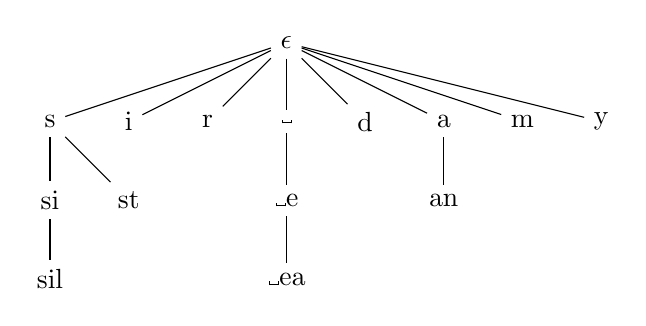
\begin{tikzpicture}
    \node (0) at (3,0) {$\epsilon$};
    
    \node (1) at (0,-1) {s};
    \node (2) at (1,-1) {i};
    \node (3) at (2,-1) {r};
    \node (4) at (3,-1) {\textvisiblespace};
    \node (5) at (0,-2) {si};
    \node (6) at (4,-1) {d};
    \node (7) at (3,-2) {\textvisiblespace e};
    \node (8) at (5,-1) {a};
    \node (9) at (1,-2) {st};
    \node (10) at (6,-1) {m};
    \node (11) at (5,-2) {an};
    \node (12) at (3,-3) {\textvisiblespace ea};
    \node (13) at (0,-3) {sil};
    \node (14) at (7,-1) {y};
    
    \draw (0) -- (1);
    \draw (0) -- (2);
    \draw (0) -- (3);
    \draw (0) -- (4);
    \draw (1) -- (5);
    \draw (0) -- (6);
    \draw (4) -- (7);
    \draw (0) -- (8);
    \draw (1) -- (9);
    \draw (0) -- (10);
    \draw (8) -- (11);
    \draw (7) -- (12);
    \draw (5) -- (13);
    \draw (0) -- (14);
    
    
\end{tikzpicture}



\subsection{LZW}


\paragraph{Basic idea} Lempel-Ziv-Welch (\Define{LZW}) is a variant of LZ78, with two main differences.
\begin{enumerate}
    \item The dictionary is \Important{initialised with all possible characters}. If we are compressing an ASCII file, then positions 0 to 255 are filled at initialisation.
    
    \item The tokens only have \Important{one field}! Since we always work with at least one character (that can always be found in the dictionary), there is no need to output the next character.
\end{enumerate}

Let us go back to our example:
\begin{quote}
    sir\textvisiblespace sid\textvisiblespace eastman\textvisiblespace easily%\textvisiblespace teases\textvisiblespace sea\textvisiblespace sick\textvisiblespace seals
\end{quote}

The dictionary is initialised with all 256 ASCII characters in positions 0 to 255, e.g. a is in position 97, b in 98, s in 115, z in 122. The first character in the string is s (in the dictionary at position 115). Since si does not appear in the dictionary, we add si to the dictionary at 256, and we continue with the character i. Again, since ir is not in the dictionary, we add ir at 257 and continue with the character r.

The dictionary (omitting positions 0 to 255) and the tokens look like this:\\
~\\
\begin{tabular}{l|l|l|l}
     Position & String & Token & What the token encodes \\
     \hline
     256 & si & 115 & s\\
     257 & ir & 105 & i\\
     258 & r\textvisiblespace & 114 & r\\
     259 & \textvisiblespace a & 32 & \textvisiblespace\\
     260 & sid & 256 & si\\
     261 & d\textvisiblespace & 100 & d\\
     262 & \textvisiblespace e & 32 & \textvisiblespace\\
     263 & ea & 101 & e\\
     264 & as & 97 & a\\
     265 & st & 115 & s\\
     266 & tm & 116 & t\\
     267 & ma & 109 & m\\
     268 & an & 97 & a\\
     269 & n\textvisiblespace & 110 & n\\
     270 & \textvisiblespace ea & 262 & \textvisiblespace e\\
     271 & asi & 264 & as\\
     272 & il & 105 & i\\
     273 & ly & 108 & l\\
        &   & 121 & y
\end{tabular}
~\\~\\
The output is then
\[
    115, 105, 114, 32, 256, 100, 32, 101, 97, 115, 116, 109, 97, 110, 262, 264, 105, 108, 121
\]

The dictionary can once again be stored as a tree, but the implementation is more complex than for LZ78. A thorough description is given in \cite[3.13.2]{Sal04}.


\subsection{Applications of LZW}

\paragraph{GIF} The ubiquitous Graphics Interchange Format (\Define{GIF}) uses a variation of LZW. It uses a dynamic, growing dictionary. It starts with the number of bits per pixel $b$: $b=2$ for monochromatic images, $b=8$ for an image with $256$ colours of shades of grey. The dictionary starts with $2^{b+1}$ entries and is doubled in size every time it fills up until it reaches $2^{12} = 4,096$ entries. At that point, the encoder may want to start a new dictionary!

GIF is not actually that good at image compression because it is unidimensional. It scans the image row after row, so it can detect similarities within a row but has trouble dealing with similarities across rows instead.

\paragraph{Limitations} One major issue of using LZW (e.g. for GIF), is that LZW is \Important{patented}. In response to that, the Portable Network Graphics format was created in the mid-90s (finalised in 96). It is based on DEFLATE (and hence LZSS) instead.

Another application of LZW was the Unix shell compression utility \texttt{compress}, that was used in the 80s. However, it was superseded by \texttt{gzip}, which typically outperforms it in terms of compression ratio.

\subsection{See further}

\paragraph{Variants} LZ78 and LZW also have a few variants, notably LZMW, LZAP and LZY. Have another look!

\paragraph{Kolmogorov complexity} The principle of Lempel-Ziv encoding is to construct a list of instructions to the decoder of the form ``Copy that string (and add that character).'' But what if we allowed any sort of instructions?

The \Define{Kolmogorov complexity} is a concept that predates Lempel-Ziv. It aims at evaluating the ``intrinsic'' complexity of a binary string. Simply put, the Kolmogorov complexity of a string $x$ w.r.t. a Turing machine $U$, denoted $K_U(x)$, is the shortest length of a program for $U$ that prints out $x$ and halts. Obviously, $K_U(x)$ is not computable. But still, we can say a lot about the Kolmogorov complexity of a random string: it's about the length of the string. Therefore, almost any string is incompressible! The study of Kolmogorov complexity and associated concepts (e.g. Solomonoff's universal probability or Chaitin's Omega number) is very intriguing but outside the scope of this course.



 \subsection{Exercises}

\begin{exercise}
Encode the string
\begin{quote}
    sir\textvisiblespace sid\textvisiblespace eastman\textvisiblespace easily\textvisiblespace teases\textvisiblespace sea\textvisiblespace sick\textvisiblespace seals
\end{quote}
with LZ78: give the dictionary table, the trie, and the output.

Encode the same string with LZW.
\end{exercise}


\begin{exercise}
Select a few (small) images, and compare the file sizes for those when saved as .bmp, .gif and .png.
\end{exercise}



\section{Context-based compression}
\label{sec:05}



\subsection{Context}

\paragraph{Context-based compression} Statistical compression (mainly for text, but not only) can be based on two properties. The first property is the frequency of symbols: the model assigns probabilities to the symbol according to their frequency in the document. 

The second one is the \Important{context}. In practice, the context a symbol consists of the $N$ symbols preceding it (note that we cannot use symbols succeeding it, as the decoder typically does not know them yet!). Context-based compression then uses the context of a symbol to \Important{predict} it (i.e. to assign it a probability). 

For instance, let's use a context of only one character. The letter h occurs in typical English text only about 5\% of the time. However, if the current symbol is t, then there is a much higher probability (around 30\%) that the next symbol will be h, since the digram th is very common in English. Note that the prediction is about assigning probabilities, not trying to figure out the next symbol exactly (which is impossible).

\paragraph{Static v Adaptive contexts} A static context-based modeler always uses the same probabilities, which are stored in some large table. Those probabilities are usually obtained by crawling through many documents (say typical English texts). There are issues with that approach, notably the fact that this might assign zero probabilities to some strings.

An adaptive context-based modeler also maintains tables of probabilities of all the possible digrams (or trigrams, or even longer $n$-grams). But this time the tables are updated all the time as more data are input, which adapts the probabilities to the particular data being compressed. \Important{Adaptive context-based compression} might be slower, but typically results in better compression.



\paragraph{Context length} One may think at first that the larger the number $N$ of symbols in the context, the better the compression. However, this might not be the case:
\begin{enumerate}
    \item A large $N$ requires to write the first $N$ symbols in plain text, which might hurt the overall compression.
    
    \item If $N$ is too large, then there are simply too many contexts, which makes storing, reading off, and writing on the table of probabilities infeasible.
    
    \item A very long context contains information about the nature of old data. It is not uncommon to have files where different parts have different symbol distributions.
\end{enumerate}
Therefore, in practice relatively small contexts are used in practice (for text compression, traditional methods use no more than 10 characters).


\subsection{PPM}

\paragraph{Basic idea} Prediction by Partial Matching (\Define{PPM}) is based on an encoder that keeps a statistical model of the text. It starts with an order-$N$ context. It searches its data structure for an occurrence of the current context $C$ followed by the next symbol $S$. If it finds no such occurrence, if decreases the order of the context to $N-1$ and tries again (the new context $C'$ is the final $N-1$ characters of $C$). It keeps \Important{shortening the context} until it is successful. 

The encoder reads the next symbol $S$ from the input stream, looks at the current order-$N$ context $C$ (the last $N$ symbols read), and based on the previous input data, computes the probability $P$ that $S$ will appear following $C$. The encoder then calls an adaptive arithmetic encoder to encode $S$ with probability $P$. If the probability $P$ is zero, the PPM encoder tries with a smaller context; it reduces the context until $P \ne 0$. What if the symbol $S$ has not been seen yet (and hence, even with order-$0$ context, we still have $P = 0$)? Then the PPM encoder enters \Define{order-$(-1)$ context}, where the probability of $S$ is simply $1/$(size of alphabet).

\begin{example} \label{example:ppm_contexts}
Let us look at the contexts and frequency counts for the following string with $11$ symbols:
\begin{quote}
    xyzzxyxyzzx
\end{quote}

\begin{tabular}{r l | r l | r l | r l | r l}
    Order 4 & & Order 3 & & Order 2 & & Order 1 & & Order 0 &   \\
    \hline
    xyzz $\to$ x & 2 & xyz $\to$ z & 2 & xy $\to$ z & 2 & x $\to$ y & 3 & x & 4\\
    yzzx $\to$ y & 1 & yzz $\to$ x & 2 & xy $\to$ x & 1 & y $\to$ z & 2 & y & 3\\
    zzxy $\to$ x & 1 & zzx $\to$ y & 1 & yz $\to$ z & 2 & y $\to$ x & 1 & z & 4\\
    zxyx $\to$ y & 1 & zxy $\to$ x & 1 & zz $\to$ x & 2 & z $\to$ z & 2 &  & \\
    xyxy $\to$ z & 1 & xyx $\to$ y & 1 & zx $\to$ y & 1 & z $\to$ x & 2 &  & \\
    yxyz $\to$ z & 1 & yxy $\to$ z & 1 & yx $\to$ y & 1 & & &  & 
\end{tabular}
\end{example}


Now, how does the encoder tell the decoder which order context it is currently using (and hence what the decoder should be using too)? The answer is to have a dedicated \Important{escape symbol}, which we'll denote esc, which should be output whenever the context size is decreased. Since this is a new character, we should also assign a probability for the escape symbol for every encountered context. There are various ways (heuristics) of assigning such probabilities. Here, we will use the so-called Method A, where the escape symbol is assigned a frequency of 1.


We are now in position to give a more explicit example. Encoding a full sequence is actually quite tedious to explain so we'll only encode a few characters. We use contexts of order at most 2. Let us consider
\begin{quote}
    this\textvisiblespace is\textvisiblespace the\textvisiblespace tithe
\end{quote}
The first few symbols are not very interesting, so let us skip forward. Let's assume we have already encoded ``this\textvisiblespace is'' and we wish to encode the next character \textvisiblespace. 

We assume the word length for arithmetic coding is six bits (we used four decimal digits in our example in Lecture \ref{sec:02}). For the sake of simplicity, we have $Low = 0$ and hence $L^* = 000000$ and $High = 1$ hence $H^* = 111111$. (As we shall see, the low and high values may vary over time.)

Here is what the table of contexts looks like\\
~\\
\begin{tabular}{lr | lr | lr}
    Order 2 &           & Order 1 & & Order 0   \\
    \hline
    th $\to$ i      & 1 & t $\to$ h & 1 & t & 1\\
    th $\to$ esc    & 1 & t $\to$ esc & 1 & h & 1 \\
    hi $\to$ s      & 1 & h $\to$ i & 1 & i & 2\\
    hi $\to$ esc    & 1 & h $\to$ esc & 1 & s & 2 \\
    \Important{is $\to$ \textvisiblespace}      & \Important{1} & i $\to$ s & 2 & \textvisiblespace & 1\\
    \Important{is $\to$ esc}    & \Important{1} & i $\to$ esc & 1 & esc & 1 \\
    s\textvisiblespace $\to$ i      & 1 & \textvisiblespace $\to$ i & 1 \\
    s\textvisiblespace $\to$ esc    & 1 & \textvisiblespace $\to$ esc & 1 \\ 
    \textvisiblespace i $\to$ s      & 1 & s $\to$ \textvisiblespace & 1 \\
    \textvisiblespace i $\to$ esc    & 1 & s $\to$ esc & 1  
\end{tabular}
~\\
~\\
The  second-order context is ``\Important{is}''. We use characters in the order of the table: the first row gives the first interval and so on. In this context, the probability of the space sign ``\textvisiblespace'' and the probability of the escape symbol esc are both equal to 1/2, and
\[
    L(\text{\textvisiblespace}) = 0, H(\text{\textvisiblespace}) = 1/2 = L(esc), H(esc) = 1. 
\]    
    The update equations for the new $Low$ and $High$ are
\begin{align*}
    Low &\gets Low + (High - Low) L(x) = 0,\\
    L^* &\gets 000000,\\
    High & \gets Low + (High - Low) H(x) = 1/2,\\
    H^* &\gets 011111.
\end{align*}
Since the first (most significant) bit of $L^*$ and $H^*$ coincide, we shift that bit out and shift $0$ into $L^*$ and shift $1$ into $H^*$. So we obtain:
\begin{enumerate}
    \item Encoded sequence for ``\textvisiblespace'': $0$,
    
    \item Lower bound $L^* = 000000$,
    
    \item Higher bound $H^* = 111111$.
\end{enumerate}

The table of contexts now becomes:\\
~\\
\begin{tabular}{lr | lr | lr}
    Order 2 &           & Order 1 & & Order 0   \\
    \hline
    th $\to$ i      & 1 & t $\to$ h & 1 & \Structure{t} & \Structure{1}\\
    th $\to$ esc    & 1 & t $\to$ esc & 1 & h & 1 \\
    hi $\to$ s      & 1 & h $\to$ i & 1 & i & 2\\
    hi $\to$ esc    & 1 & h $\to$ esc & 1 & s & 2 \\
    is $\to$ \textvisiblespace      & 2 & i $\to$ s & 2 & \textvisiblespace & 2\\
    is $\to$ esc    & 1 & i $\to$ esc & 1 & esc & 1 \\
    \Structure{s\textvisiblespace $\to$ i}      & \Structure{1} & \Structure{\textvisiblespace $\to$ i} & \Structure{1} \\
    \Structure{s\textvisiblespace $\to$ esc}    & \Structure{1} & \Structure{\textvisiblespace $\to$ esc} & \Structure{1} \\ 
    \textvisiblespace i $\to$ s      & 1 & s $\to$ \textvisiblespace & 2 \\
    \textvisiblespace i $\to$ esc    & 1 & s $\to$ esc & 1  
\end{tabular}
~\\
~\\
The next symbol is ``t''. The second-order context is ``\Structure{s\textvisiblespace }''. Since ``t'' has zero frequency in this context, we need to encode the escape symbol. By a similar argument as above, we obtain
\begin{enumerate}
    \item Encoded escape symbol sequence: $1$,
    
    \item Lower bound $L^* = 000000$,
    
    \item Higher bound $H^* = 111111$.
\end{enumerate}
We need to look at the first-order context, which is ``\Structure{\textvisiblespace}''. Again, ``t'' does not appear with this context, so we encode another escape symbol. We obtain
\begin{enumerate}
    \item Encoded escape symbol sequence: $1$,
    
    \item Lower bound $L^* = 000000$,
    
    \item Higher bound $H^* = 111111$.
\end{enumerate}
We need to look at the zero-th order context. This time, ``t'' has already appeared, and is assigned the interval $[0, 1/9 )$. We then have 
\begin{align*}
    Low &\gets Low + (High - Low) L(x) = 0,\\
    L^* &\gets 000000,\\
    High & \gets Low + (High - Low) H(x) = 1/9,\\
    H^* &\gets 000111.
\end{align*}
Since the three leftmost bits are equal, we shift them out. We finally obtain
\begin{enumerate}
    \item Encoded sequence: for ``t'': $000$,
    
    \item Lower bound $L^* = 000000$,
    
    \item Higher bound $H^* = 111111$.
\end{enumerate}
So, to encode ``\textvisiblespace t'', we have transmitted $011000$.

Note that there would be a slight difference in practice: to keep everything integral, we would use $High = 63$, $Low = 0$ and perform an update of the form
\begin{align*}
    Low &\gets Low + \left\lfloor (High - Low + 1) \frac{ 1 }{ 9 }  \right\rfloor  = 0 = 000000\\
    High & \gets High + \left\lfloor (High - Low + 1) \frac{ 1 }{ 9 }  \right\rfloor - 1  = 6 = 000110
\end{align*}
Then we would have: Higher bound $H^* = 110111$.


\paragraph{Methods B and C} Two other main ways of assigning frequencies to the escape symbols aim to make the escape symbol more probable, which typically reduces the size of the resulting sequence for that symbol. The main idea is that if a context is followed by many different characters, then you are likely to encounter yet another character following that same context. For instance, think of the context ``s'' in English, which can be followed by virtually any other letter. \Important{Methods B and C} give the escape symbol a count equal to the number of symbols following the context; Method B then subtracts the count of every other symbol by one, while Method C does not amend those.


\subsection{See further}

\paragraph{RAR} The main application of PPM is in the Roshal Archive (\Define{RAR}) file format. 


\paragraph{Context mixing} In \Define{context mixing}, the next-symbol predictions of two or more statistical models are combined to yield a prediction that is often more accurate than any of the individual predictions. The \Important{PAQ} series of data compression programs use context mixing; they are the cutting edge in lossless compression in terms of compression ratio (at the expense of speed and memory usage) \cite{KF11}. 

Note that the problem of mixing different contexts is a very challenging issue in machine learning; that could be a very interesting topic for a project...


\paragraph{BWT} The Burrows-Wheeler transform (\Define{BWT}) is a very clever way of converting a list of symbols into one that is much more structured. You only need a little more information to make sure that the transform does not lose any information. By structured, we mean that it is ``almost sorted.'' After the transform, one can use very simple techniques to efficiently encode the structured list. Unfortunately, BWT-based compression requires to scan and to manipulate the whole message, which is an important drawback compared to the adaptive PPM.


\subsection{Exercises}


\begin{exercise} \label{exercise:ppm_contexts}
Update the table in Example \ref{example:ppm_contexts} if the following character is x.
\end{exercise}

\begin{exercise}
Finish the encoding of the sequence ``this\textvisiblespace is\textvisiblespace the\textvisiblespace tithe''. To update $High$ and $Low$, you may use our simple technique based on rational numbers, or use the version with integers instead.
\end{exercise}


\bibliographystyle{plain}
\bibliography{references}


\end{document}
